
\newcommand\upquote[1]{\textquotesingle#1\textquotesingle}


\section{Introduction}

In nature, ants scavenge for food as a swarm. They choose their paths from the nest based on pheromone density, favoring paths with higher concentrations of pheromone.  Individuals lay pheromone trails upon finding food, allowing other members of their colony to passively follow them to the food source.  Because paths leading to food have higher pheromone density, increasing numbers of ants choose these successful paths.  As a result, ant trails transition over time from random paths to streamlined routes.  This organization and appearance of patterns over time is an example of \textbf{emergence},  the process by which complex systems and patterns arise from a multiplicity of simple systems.

Ant feeding patterns lend themselves to simulation with \textbf{agent-based models}, which simulate  the actions and interactions of autonomous agents  to assess their effects on the system as a whole.  When we model ant feeding patterns, each ant is an agent in the model, a self-governing individual that makes decisions based on its surroundings.  When simulating large numbers of ants,  behavior emerges that is reflective of ant behavior in the natural world.  Beyond being intrinsically fascinating, such models have applications in the ``real world'' in areas ranging from city planning to film production.  We will discuss the application of agent-based models to the entertainment industry later in the paper.

\section{Model Overview}

We can see one example of an agent-based model in Deneuborg et al.'s 1989 paper \emph{The Blind Leading the Blind: Modeling Chemically Mediated Army Ant Raid Patterns}, freely available at  \url{http://www.ulb.ac.be/sciences/use/publications/JLD/80.pdf}.

The premise of the model is that as ants move around they lay pheromone, which increases the likelihood that other ants will follow the same path. Ants that have found food lay more pheromone than ants that haven't, making it likely that other ants will follow their paths to find more food. 

The ants live in a two-dimensional world of discrete points arranged in a grid. At each step of the model, each ant has a certain probability of moving to one of two neighboring coordinates in the direction the ant is facing, away from the nest---forward left or forward right. All of the ants start out in a corner of the world, which we call the \emph{nest}, and at each time step of the simulation, we add more ants to the nest. This leads to a constant stream of outgoing ants.

\begin{figure}
\centerline{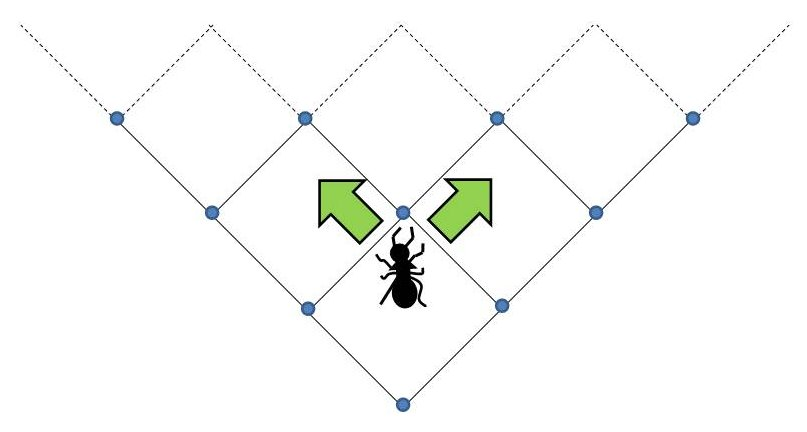
\includegraphics[width=3.0in]{figs/antchoice.jpg}}
\caption{In the model, ants live in a grid and face away from the nest. At each time step, they can move forward left or forward right.\label{fig.antchoice}}
\end{figure}

Once an ant has found food, it turns back towards the nest. It obeys the same rules for motion---that is, in each time step, its choice to move either forward left or forward right is influenced by the amounts of pheromone it sees, except now, these choices take it back towards the nest. Also, after moving, the ant lays more pheromone than it did while foraging for food. This significantly increases the probability that other foraging ants will follow its path to find, potentially, more food.

In its starting configuration, each point in the world has a chance of containing food. Once this starting condition has been set, we let the simulation run for about 1000 time steps, and plot the result. You can see the plot of one such simulation in Figure~\ref{fig.plot}, which is similar to what Deneuborg et al. claim actual army ant foraging patterns look like in their paper because observable ant trails have emerged.

\begin{figure}[ht]
\centerline{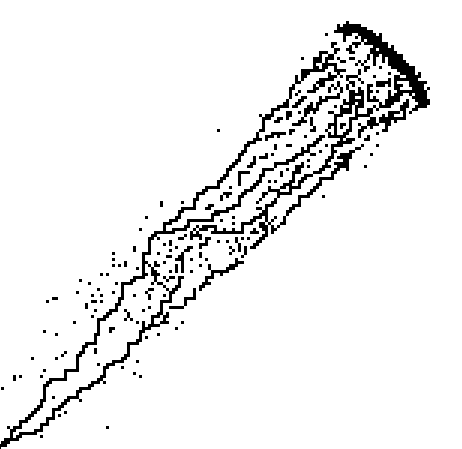
\includegraphics[width=3.0in]{figs/plot.png}}
\caption{Plot of our simulation after 1000 time steps.\label{fig.plot}}
\end{figure}

\begin{ex}
Download the code for \texttt{ants.py}, our simulation, available at \url{thinkcomplex.com/ants.py}.  Run it for 1000 time steps and see if your results look similar to Figure~\ref{fig.plot}. The simulation can be computationally intensive, and 1000 time steps took about 1.5 minutes to run on our machine---be patient!
\end{ex}


\section{API design}

A major challenge of writing a simulation such as this is coming up with classes that are easy for human readers of the code to understand, as well as implementing data structures that allow the code to execute efficiently.

One way to break up a model into classes is to list the main nouns you use when describing the model, and then represent the most prominent of those nouns as classes. In the case of our model, we have the World, which contains Ants along with Locations that may or may not contain food.

The next step is to decide what information about the current state of the model an instance of each class will be responsible for knowing. In our case, the behavior of the World is defined by what the Ants and Locations can do, so it makes sense to design our classes bottom-up and consider the World only once we have at least a tentative idea for the methods and attributes of Ants and Locations.

The most important piece of information that Ants know is where they are located in the World; as such, each ant has the attributes \texttt{x} and \texttt{y} to keep track of its current coordinates. Also, each Ant keeps track of whether or not it is currently carrying food, so we define \texttt{has\_food} for this purpose.

Note that Ants know only local information about the World; keeping track of all the Ants will be the job of the World object itself.

Knowing that the World will have to interact with individual Ants, we define two methods inside the Ant class that will get called by the World:

\begin{itemize}
 \item \texttt{move}: Figures out whether the Ant will move this turn, and if so, moves the Ant accordingly.
 \item \texttt{getPos}: Returns the current coordinates of this Ant.
\end{itemize}

The Ant class contains numerous other methods, but these are intended for internal use by each Ant object only, and not by the World. For example, the methods \texttt{will\_move} and \texttt{will\_go\_right} determine whether or not the Ant will move this turn and if so, whether it will move forward right or forward left, but these methods are only ever called by the Ant's \texttt{move} method. Similarly, \texttt{move} is the only method that calls \texttt{lay\_pheromone}, which increases the pheromone count at the Ant's current Location in the World.

Locations know even less than Ants; each Location only keeps track of the food and pheromone it contains, using attributes called \texttt{food} and \texttt{pheromone}, respectively. As far as methods go, a Location only has short accessor methods that Ants and the World use to modify the Location's food and pheromone amounts.

Note that unlike Ants, Locations do not keep track of their coordinates on the map. While having them do so might make sense at first, we decided against it because a Location's coordinates never change; since the World must already keep track of each Location's coordinates so it can access the correct Location given its x and y positions, having the Location also keep track of its position would be redundant.

The World is the ``meat'' of our simulation---it is where most of the work gets done. The World is only ever instantiated once, and this instance keeps track of all existing Ants and Locations. 

The World has methods for controlling the overall state of the simulation. The World's \texttt{move\_ants} method advances the simulation by one time step by calling every existing Ant's \texttt{move} method, changing the \texttt{ants} attribute to reflect the Ants' new positions, and evaporating a certain proportion of pheromone from each Location. Other methods include \texttt{add\_ants}, which adds a specified number of ants to the nest, \texttt{place\_food}, which fills each Location on the map with food at a certain probability, and \texttt{get\_location}, which returns a reference to the Location at the given coordinates.

\section{Sparse matrices}

The group of Locations that make up our World is implemented as a \textbf{sparse matrix}. What this means is that Locations don't exist in our representation until they are needed; the World's \texttt{get\_location} method is responsible for fetching either the existing Location at the given coordinates, or creating a new Point if one doesn't already exist there. An alternate implementation would be a \textbf{dense matrix}, which would be a two-dimensional array---a list of lists---of all Locations in the world. In our case, a sparse matrix has two main advantages over a dense matrix:

\begin{itemize}
\item Since most of the World is empty most of the time, it's more memory-efficient to only keep track of those Locations that aren't empty.
\item A sparse matrix, unlike a dense matrix, doesn't have set dimensions. This means that in our implementation, an Ant is free to wander off in any direction with no additional development cost to us as programmers, whereas in a dense matrix if an Ant were to walk outside the dimensions of the matrix, the dimensions would have to be expanded in a developmentally costly operation.
\end{itemize}

\section{wx}

We use the \texttt{wx} Python package to plot a picture of the ants after the simulation finishes running. 

Our code defines a class called \texttt{AntPlot} which is responsible for taking the World and popping up a \texttt{wx} window that plots the ants as seen in Figure~\ref{fig.plot}:

\begin{verbatim}
class AntPlot:
    def __init__(self, world):
        self.world = world
        self.app = wx.PySimpleApp()
        self.w = 500
        self.h = 500
        self.frame = wx.Frame(None, -1, 'Ant Plot', size=(self.w, self.h))
        self.canvas = FloatCanvas(self.frame, -1)
        
    
    def draw(self):
        positions = self.world.get_ant_dict()
        for pos in positions:
            x, y = pos
            x -= self.w / 2
            y -= self.h / 2
            self.canvas.AddPoint((x, y))
        self.frame.Show()
        self.app.MainLoop()
\end{verbatim}

The specific widget we use to accomplish the plotting is a \texttt{FloatCanvas}. Most canvases in GUI libraries define the point (0, 0) as the upper left corner of the canvas and have x increase to the left and y increase down, but the coordinates in the \texttt{FloatCanvas} work like in math---(0, 0) is defined as the middle, and y increases up. This allows us to write simpler code because we don't have to transform our coordinates to the canvas's system like we would have to for a traditional canvas.

Our \texttt{AntPlot} class serves as somewhat of a ``hello world'' application for \texttt{wx}---all it does is pop up a single window and some plotting. If you are interested in exploring \texttt{wx} further, this class might be a good starting point.


\begin{ex}
Try altering the pheromone amounts in the model.  What happens when Ants only lay pheromone when leaving the nest? When returning? What happens when Ants lay significantly more or less pheromone than currently? Are there any boundary conditions?
\end{ex}

\begin{ex}
Different species of ants have different patterns of food locations. In \texttt{ant.py}, each Location has a 50\% probability of containing one particle of food.  What happens when each Location has a 1\% probability of containing 50 pieces of food?
\end{ex}

\begin{ex}
So far, we have only considered scenarios involving one nest of ants.  What happens when we consider multiple nests? Pick a value d and modify the code such that Ants spawn at (0, d) and (d, 0) in addition to (0,0).  Do the trails of ants converge, or do they all remain distinct? Try keeping track of the amount of food that has been collected in each nest. Does any one of the nests do better than the others?
\end{ex}

\begin{ex}
Previously, we have assumed that all ants lay the same quantity of pheromone as other ants.  Revisiting our three-nest scenario, what happens when ants from one nest lay slightly higher amounts of pheromone than those from the other nests?
\end{ex}



\section{Applications}

Agent-based models have numerous applications in the ``real world'', from modeling traffic patterns to creating realistic battle simulations.  The entertainment industry has begun using agent-based models to simulate crowds in films, games, and advertisements that would have previously been infeasible to create.  Modeling is far more scalable than filming; that is, it is much easier to model a crowd of a hundred thousand people than it is to recruit a hundred thousand extras.  The application of agent-based models to the entertainment industry has changed the nature of film as we know it by allowing for the creation of large-scale, visually stunning sequences.

The \emph{Lord of the Rings} trilogy is the canonical example of films only possible with the use of agent-based models.  The current industry-standard software, called Massive, was originally developed to simulate life-like battle sequences in the trilogy.   Massive has since been used in a wide variety of films, for battle sequences in movies like \emph{Chronicles of Narnia} and \emph{300}, as well as for more benign crowd simulations in films such as \emph{Happy Feet} and \emph{Avatar}.

In \emph{Lord of the Rings}, developers were tasked with creating battles with hundreds of thousands of soldiers from a variety of races with many different fighting techniques.  In order to create these battles, they implemented a simulation wherein each fighter was an agent.  Each agent had about 200 possible motions it could perform which were animated using motion-capture.  Within its ``brain'', the agent chose from the possible responses based on logic and probabilities.  Different races within the battles, such as elves, orcs and men, were based on the same ``master agent'' but had different weapons, abilities and programmed attack responses.  

Simulating thousands of agents in tandem allowed for exceptionally complex and sometimes unpredictable battle sequences.  The results sometimes surprised even Massive's developers---in one shot of the prologue battle scene, a number of agents fled the battle.  The agents were not programmed to flee; that is, fleeing was not one of their ``options'' when evaluating the situation to decide which action to perform.  Rather, this decision came about based on their evaluation of location and determination to run from enemies and not fight---an emergent behavior. This unexpected action, which would be realistic in an actual battle scenario, speaks to the power of agent-based models.  

The use of agent-based models allowed battle sequences to be re-simulated and tinkered with until results were satisfactory.  This freedom allowed directors to experiment far more than would have been possible with casted battles.

You may be wondering how \emph{Lord of the Rings} relates to ant trails.  Clearly, the models used in the films are far more complicated than those we used to simulate ant trails; however, their results are further proof of the same concept.  Like the agents in \emph{Lord of the Rings}, our ants were given relatively simple commands from which complex behavior evolved.  Moreover, this behavior was believable and true to the natural world. 

















